\documentclass[../sparc.tex]{subfiles}
\usetikzlibrary{math}
\graphicspath{{\subfix{../images/}}}
\begin{document}

%%%%%%%%%%%%%%%%%%%%%%%%%%%%%%%%%%%%%%%%%%%%%%%%%%%%%%%%%%%%%%%%%%%%%%%%%%%%%%%%
\section{Анимация}
\index{Разработка игр!Анимация}

В данном разделе мы сделаем так, чтобы игрок поворачивался в ту сторону, в
которую он идёт.  Для этого нам необходимо сделать три варианта ``модели''
персонажа: первая, где персонаж стоит на месте; вторая, где персонаж смотрит
вправо и третья, где персонаж смотрит влево.

Чтобы съэкономить драгоценные ячейки под собственные в памяти дисплея, мы будем
использовать один и тот же код символа, меняя при этом отрисовку этого символа.

%%%%%%%%%%%%%%%%%%%%%%%%%%%%%%%%%%%%%%%%%%%%%%%%%%%%%%%%%%%%%%%%%%%%%%%%%%%%%%%%
\subsection{Добавление необходимых символов}

У персонажа нашей игры будет три состояния: перемещение влево (``LEFT''),
бездействие (``IDLE''), перемещение вправо (``RIGHT'').  Для каждого из этих
состояний необходимо сделать ``текстуру'', которая будет применяться
(см. рис. \ref{fig:game-dev-player-textures}.)

\begin{figure}[ht]
  \centering
  \def \offsetLeft{0.0}
  \def \offsetIdle{3.5}
  \def \offsetRight{7.0}
  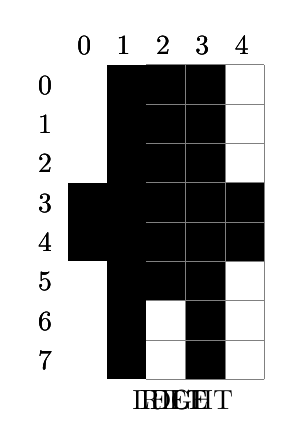
\begin{tikzpicture}
    %% Left.
    %% 0
    \fill[black] (\offsetLeft + 0.5, 0) rectangle (\offsetLeft + 2.0, -0.5);
    %% 1
    \fill[black] (\offsetLeft + 1.0, -0.5) rectangle (\offsetLeft + 2.0, -1.0);
    %% 2
    \fill[black] (\offsetLeft + 1.5, -1.0) rectangle (\offsetLeft + 2.0, -1.5);
    %% 3
    \fill[black] (\offsetLeft + 0.0, -1.5) rectangle (\offsetLeft + 2.0, -2.0);
    %% 4
    \fill[black] (\offsetLeft + 1.5, -2.0) rectangle (\offsetLeft + 2.0, -2.5);
    %% 5
    \fill[black] (\offsetLeft + 1.0, -2.5) rectangle (\offsetLeft + 2.0, -3.0);
    %% 6
    \fill[black] (\offsetLeft + 2.0, -3.0) rectangle (\offsetLeft + 1.5, -3.5);
    \fill[black] (\offsetLeft + 1.0, -3.0) rectangle (\offsetLeft + 0.5, -3.5);
    %% 7
    \fill[black] (\offsetLeft + 2.0, -3.5) rectangle (\offsetLeft + 1.5, -4.0);
    \fill[black] (\offsetLeft + 1.0, -3.5) rectangle (\offsetLeft + 0.5, -4.0);
    \draw[step=0.5cm,gray,very thin] (\offsetLeft, -4.0) grid (\offsetLeft + 2.5, 0);
    %% Numbers
    \foreach[count=\n from 0] \x in {0.0, 0.5, ..., 2.0} {
      \draw (\offsetLeft + \x cm, 0 cm) node[anchor=south west] {$\n$};
    }
    \foreach[count=\n from 0] \y in {-0.5, -1.0, ..., -4.0} {
      \draw (\offsetLeft - 0.5 cm, \y cm) node[anchor=south west] {$\n$};
    }
    \draw (\offsetLeft + 0.7, -4.5) node[anchor=south west] {LEFT};

    %% Idle.
    %% 0
    \fill[black] (\offsetIdle + 2.0, 0) rectangle (\offsetIdle + 0.5, -1.0);
    %% 2
    \fill[black] (\offsetIdle + 1.0, -1.0) rectangle (\offsetIdle + 1.5, -1.5);
    %% 3
    \fill[black] (\offsetIdle + 0.5, -1.5) rectangle (\offsetIdle + 2.0, -2.0);
    %% 4
    \fill[black] (\offsetIdle + 2.0, -2.0) rectangle (\offsetIdle + 2.5, -2.5);
    \fill[black] (\offsetIdle + 1.5, -2.0) rectangle (\offsetIdle + 1.0, -2.5);
    \fill[black] (\offsetIdle + 0.5, -2.0) rectangle (\offsetIdle + 0.0, -2.5);
    %% 5
    \fill[black] (\offsetIdle + 0.5, -2.5) rectangle (\offsetIdle + 2.0, -3.0);
    %% 6
    \fill[black] (\offsetIdle + 2.0, -3.0) rectangle (\offsetIdle + 1.5, -3.5);
    \fill[black] (\offsetIdle + 1.0, -3.0) rectangle (\offsetIdle + 0.5, -3.5);
    %% 7
    \fill[black] (\offsetIdle + 2.0, -3.5) rectangle (\offsetIdle + 1.5, -4.0);
    \fill[black] (\offsetIdle + 1.0, -3.5) rectangle (\offsetIdle + 0.5, -4.0);
    \draw[step=0.5cm,gray,very thin] (\offsetIdle, -4.0) grid (\offsetIdle + 2.5, 0);
    %% Numbers
    \foreach[count=\n from 0] \x in {0.0, 0.5, ..., 2.0} {
      \draw (\offsetIdle + \x, 0) node[anchor=south west] {$\n$};
    }
    \foreach[count=\n from 0] \y in {-0.5, -1.0, ..., -4.0} {
      \draw (\offsetIdle - 0.5, \y ) node[anchor=south west] {$\n$};
    }
    \draw (\offsetIdle + 0.8, -4.5) node[anchor=south west] {IDLE};

    %% Right.
    %% 0
    \fill[black] (\offsetRight + 0.5, 0) rectangle (\offsetRight + 2.0, -0.5);
    %% 1
    \fill[black] (\offsetRight + 0.5, 0) rectangle (\offsetRight + 1.5, -1.0);
    %% 2
    \fill[black] (\offsetRight + 0.5, -1.0) rectangle (\offsetRight + 1.0, -1.5);
    %% 3
    \fill[black] (\offsetRight + 0.5, -1.5) rectangle (\offsetRight + 2.5, -2.0);
    %% 4
    \fill[black] (\offsetRight + 0.5, -2.0) rectangle (\offsetRight + 1.0, -2.5);
    %% 5
    \fill[black] (\offsetRight + 0.5, -2.5) rectangle (\offsetRight + 1.5, -3.0);
    %% 6
    \fill[black] (\offsetRight + 2.0, -3.0) rectangle (\offsetRight + 1.5, -3.5);
    \fill[black] (\offsetRight + 1.0, -3.0) rectangle (\offsetRight + 0.5, -3.5);
    %% 7
    \fill[black] (\offsetRight + 2.0, -3.5) rectangle (\offsetRight + 1.5, -4.0);
    \fill[black] (\offsetRight + 1.0, -3.5) rectangle (\offsetRight + 0.5, -4.0);
    \draw[step=0.5cm,gray,very thin] (\offsetRight, -4.0) grid (\offsetRight + 2.5, 0);
    %% Numbers
    \foreach[count=\n from 0] \x in {0.0, 0.5, ..., 2.0} {
      \draw (\offsetRight + \x, 0) node[anchor=south west] {$\n$};
    }
    \foreach[count=\n from 0] \y in {-0.5, -1.0, ..., -4.0} {
      \draw (\offsetRight - 0.5, \y) node[anchor=south west] {$\n$};
    }
    \draw (\offsetRight + 0.8, -4.5) node[anchor=south west] {RIGHT};
  \end{tikzpicture}
  \caption{Три варианта изображение игрока: смотрящий влево (``LEFT''),
    бездействующий (``IDLE'') и смотрящий вправо (``RIGHT''.)}
  \label{fig:game-dev-player-textures}
\end{figure}

%%%%%%%%%%%%%%%%%%%%%%%%%%%%%%%%%%%%%%%%%%%%%%%%%%%%%%%%%%%%%%%%%%%%%%%%%%%%%%%%
\subsection{Реализация анимации}

Для того, чтобы реализовать анимацию поворота игрока в сторону направления
движения, нам необходимо добавить вызов \texttt{createChar} непосредственно в
код функции \texttt{loop}.

Первым делом после вызова \texttt{map\_show} мы добавим перезапись символа игрока
для того, чтобы вернуть его в бездействующее положение.

\begin{minted}{cpp}
  void loop() {
    map_show();
    lcd.createChar(PLAYER, player_idle_image);
    // ...
  }
\end{minted}

Затем мы должны перезаписывать символ игрока каждый раз, когда мы видим, что
нажата кнопка вправа или влево.

\begin{minted}{cpp}
  void loop() {
    map_show();
    lcd.createChar(PLAYER, player_idle_image);

    if (digitalRead(BUTTON_R) == LOW) {
      lcd.createChar(PLAYER, player_right_image);
      player_x++;
    }
    if (digitalRead(BUTTON_L) == LOW) {
      lcd.createChar(PLAYER, player_left_image);
      player_x--;
    }
  }
\end{minted}

\end{document}
